\documentclass[10pt,letterpaper]{article}

\usepackage{cvpr}
\usepackage{times}
\usepackage{epsfig}
\usepackage{graphicx}
\usepackage{amsmath}
\usepackage{amssymb}
\usepackage[pagebackref=true,breaklinks=true,letterpaper=true,colorlinks,bookmarks=true,bookmarksnumbered=true,hypertexnames=false,linkbordercolor={0 0 1}]{hyperref}
% Include other packages here, before hyperref.

% If you comment hyperref and then uncomment it, you should delete
% egpaper.aux before re-running latex.  (Or just hit 'q' on the first latex
% run, let it finish, and you should be clear).
%\usepackage[pagebackref=true,breaklinks=true,letterpaper=true,colorlinks,bookmarks=false]{hyperref}

\cvprfinalcopy % *** Uncomment this line for the final submission

\def\cvprPaperID{****} % *** Enter the CVPR Paper ID here
\def\httilde{\mbox{\tt\raisebox{-.5ex}{\symbol{126}}}}

% Pages are numbered in submission mode, and unnumbered in camera-ready
\ifcvprfinal\pagestyle{empty}\fi
%\setcounter{page}{1}
\begin{document}

%%%%%%%%% TITLE
\title{Automatic Face Editing on a Morphable Model}

\author{Han Li\\
Department of Computer Sciences\\
University of Wisconsin-Madison\\
{\tt\small hli337@wisc.edu}
% For a paper whose authors are all at the same institution,
% omit the following lines up until the closing ``}''.
% Additional authors and addresses can be added with ``\and'',
% just like the second author.
% To save space, use either the email address or home page, not both
\and
Wentao Wu\\
Department of Computer Sciences\\
University of Wisconsin-Madison\\
{\tt\small wwu69@wisc.edu}
}

\maketitle
%\thispagestyle{empty}

%%%%%%%%% ABSTRACT
\begin{abstract}
%Describe   the goal of the project, the data/device as well as which techniques you plan to use.
With the unprecedented and exponentially increasing of web images and videos,  there is a growing concern of online iconographic privacy. Thus, editing and rewriting these image-based media resources is becoming an interesting and urgent task. In this project, we are planning to implement automatic face editing in a resource (image or video) based on face morphing and blending from an existing facial data collection. The anticipated procedure consists of three steps: (1) face alignment based on Active Shape Models and facial expression recognition, (2) face morphing by the 2D morphable model, and (3) face blending with color and illumination adjusting.

\end{abstract}

%%%%%%%%% BODY TEXT
\section{Introduction}
\label{sect:intro}

%Outline the background of your project, explain why it  is important. 
%
%Describe your project goals.  Be specific.  Describe what the inputs to the system are, and what the outputs will be.
% 
%Brief description of your approach. You may use figures to outline the framework as shown in Fig. \ref{fig:teaser}.
With the unprecedented and exponentially increasing of high-definition web images and videos, online iconographic privacy is becoming a severe problem and concerned by more and more people. For example, online systems such as Google Street View allow users to browse photos of public images possibly containing many people who might not consent to be photographed. Thus, it becomes more and more urgent and popular to develop face editing techniques to alleviate this problem. In this project, we are planning to implement a face editing method based on a 2D morphable model for image and video facial information hiding. Given a set of facial image collection containing faces of different poses and expressions and a target resource (image or video), Fig. \ref{fig:pipeline} shows the pipeline of our procedure: (1) face detection and alignment based on Active Shape Models integrating the facial expression recognition procedure; (2) face morphing by the 2D morphable model, and (3) face blending with possible color and illumination adjusting. Since the many of the previous methods haven't cared much about the facial expressions, the contribution of this project would be integrating the facial expression recognition into the face editing procedure and substituting a new face with a similar expression.


\begin{figure}[th]
\begin{center}
 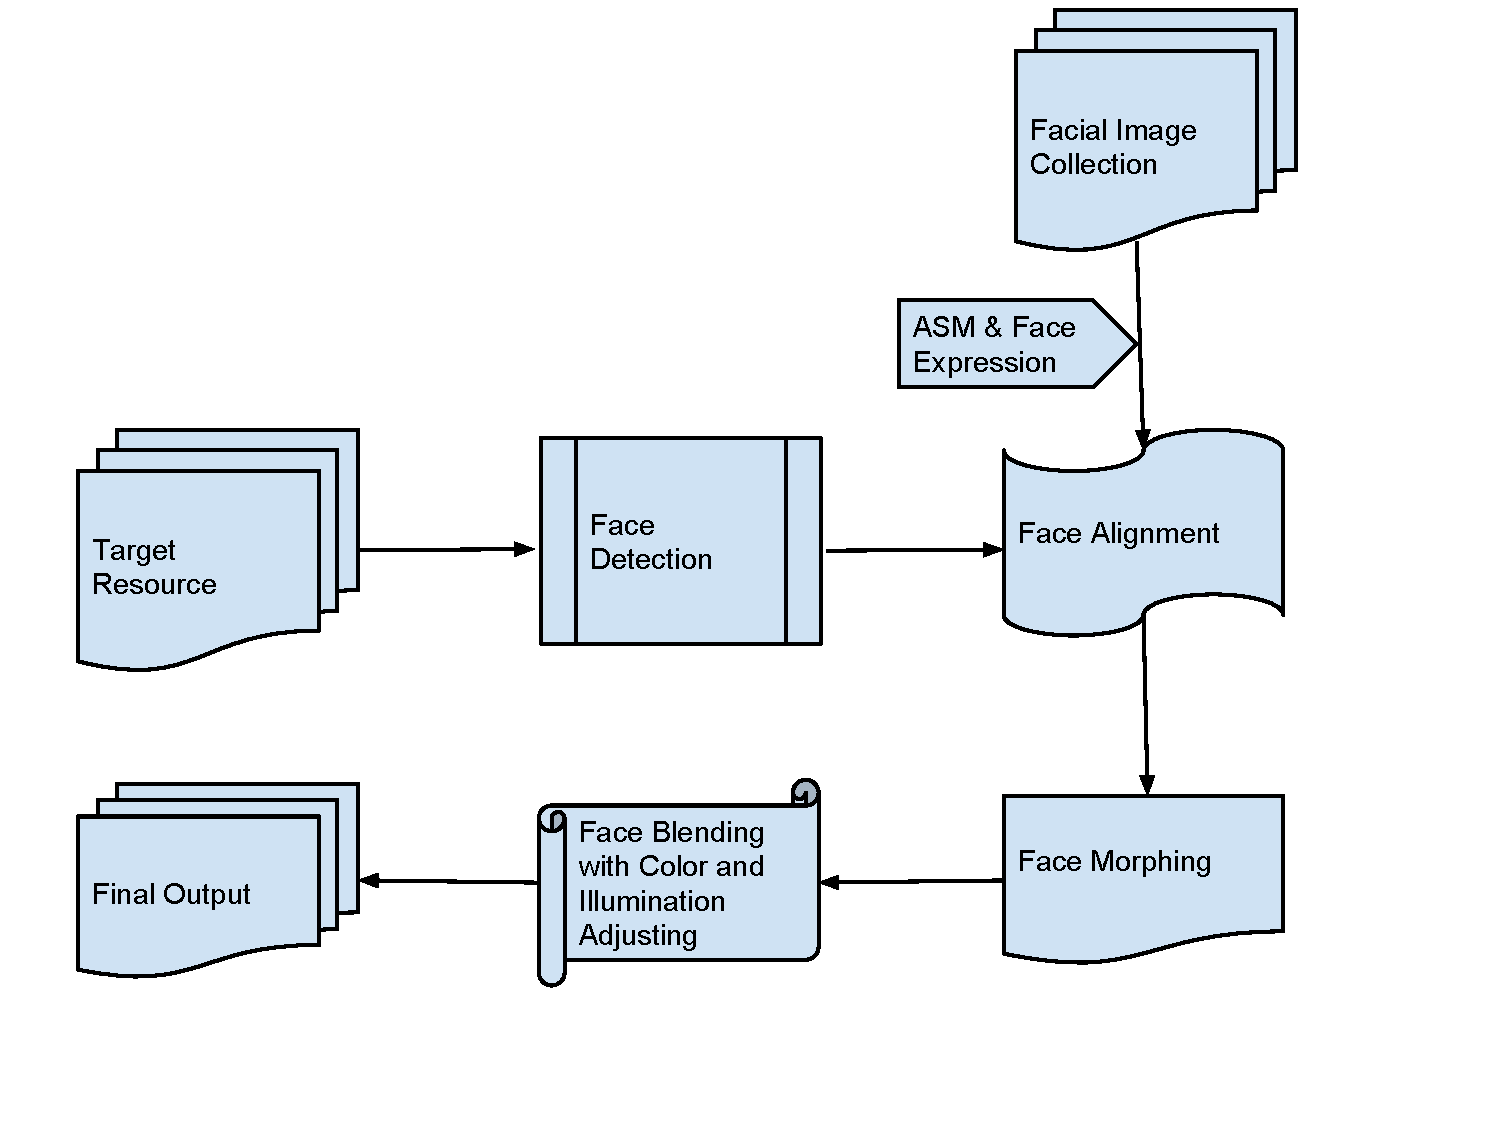
\includegraphics[width=0.5\linewidth]{fig/Flowchart.pdf} 
\end{center}
   \caption{The pipeline of the face editing procedure.}
\label{fig:pipeline}
 
\end{figure}

 
 \section{Related Work}

%Discuss related work to your project, give those references here \cite{Alpher03,Alpher04,Authors06}. 

%Briefly describe what is done in each reference, what are their limitations, and what you will do differently.
Our project is most related to Min's work \cite{min2010automatic}. They proposed an automatic face
replacement approach in video based on 2D Morphable model. This approach includes three main modules: face alignment, face morph, and face fusion. They use the Active Shape Models (ASM) for face alignment. They also consider color and lightning adjustment to keep consistent. Their approach is fully automatic without user interference, and generates natural and realistic results. Furthermore, as they use 2D model, their algorithm is also efficient. However, they don't consider facial expression. The tolerance to pose and expression variance is limited by ASM.

Liang \cite{liang2009image} proposed a video face replacement system which allows replacing target human face from
target video with source face in source video. For each target face in target video, they select the best candidate face with similar facial expression. Finally, they blend candidate replacement to target video. In their approach, however, they require the target video should have similar face expression and pose with the source video. 

Similar to Liang's work, Dale \cite{dale2011video} also proposed an algorithm to provides face replacement in target video from source video. They tracks both faces in target and source video using multilinear model. By the tracked 3D geometry, source face is warped to target face in every frame of video. But, their tracking algorithm is based on optical flow, so the light should change slowly in the video.

Afifi \cite{afifi2014video} presented a system for video face replacement that requires only two videos of a source actor and a target actor using only a single digital camera. They could generate realistic results without using special equipment and 3D model. Also, they use a new face blending technique based on poisson blending. But their algorithm only works for fixed pose, i.e. front face.

Instead of using source video, Cheng \cite{cheng20093d} uses only two face pictures: one frontal view and one profile view. First, they use these two images to construct 3D face model. Then, they track the faces in the video and project the source face model to align and replacement the faces in target video. However, the tolerance to the pose is limited to robustness of their alignment algorithm.

A. Niswar \cite{niswar2012face} proposed a system where one image is required to replace the faces in target video. Also, the image is not limited to a specific pose. There are four steps in their approach: 3D face reconstruction, 3D face animation, feature points tracking, 2D projection with blending. Their approach, however, has high complexity and hence high time consuming. 
%-------------------------------------------------------------------------
\section{Problem Description and Techniques to Be Used}

%Describe your project goal in detail. You are also encouraged to apply computer vision techniques on the open problems
%in your own research areas.
%
%Outline techniques you plan to use for your problem.
The basic steps of the method have been outlined in Section \ref{sect:intro}. Given a face image collection{\footnote[1]{this set of images could be captured easily.}} $F = \{f_1, f_2, \dots, f_n\}$ with $n$ faces of different poses and facial expressions and a target resource with a list of face sequence $L_{F,old} = \langle l_1, l_2, \dots, l_m \rangle$ with $m$ faces that would be recognized by the facial detection method, our goal is that for each $L_{F, old}(i)$, we would find the best face $f_{best(i)} \in F$ such that after performing morphing and blending, the new face
$L_{F, new}(i) = Blend(Morph(L_{F, old}(i)))$ looks natural to human judgements. The methods and techniques used during the procedure would be face detection, alignment, morphing, blending model, and color and illumination adjusting methods.

\section{Experimental Evaluation}
 

%Describe the data you plan to use, the baselines you want to compare (if applicable), and the evaluation metric.

%If you plan to use some special equipment, mention it here.   We may be able to help with servers, extra cameras, etc.
We plan to focus our attention on image face editing firstly and then extend the method to edit videos. The source face images would be captured manually with many different poses and expressions, and the target resources would be captured from the Internet. Since there is no good quantitative evaluation method, we would evaluate the performance of our model qualitatively based on human judgements.

 
%------------------------------------------------------------------------
\section{Conclusion and Discussion}
 
%Breakdown--what will each team-member do? Time-line of your project? Ideally, everyone should do something imaging/vision related (it's not good for one team member to focus purely on user-interface, for instance).

%You full proposal should be two pages excluding references using this template.
Han Li: focus on face detection and alignment.

Wentao Wu: focus on face morphing and blending.

We plan to use one week for related methods understanding, two weeks for face editing implementation, and one week for debugging and improving. We would provide demos for the performance evaluation.

\clearpage

{\small
\bibliographystyle{ieee}
\bibliography{proposal}
}

\end{document}


